\documentclass[10pt]{article}
\usepackage{paper_style}

\PaperTitle{%
  1行目のタイトル\\
  2行目のタイトル
}
\PaperAdvisor{指導教員　教授　氏名，助教　氏名}
\PaperStudent{学籍番号　氏名}

\begin{document}
\MakePaperTitle

\begin{PaperBody}

\section{研究背景}\label{sec:background}
ここに研究背景を書く．必要に応じて，先行研究を \papercite{1} の形で参照する．

\section{研究目的}\label{sec:purpose}
ここに研究目的を書く．

\section{研究目標}\label{sec:goal}
ここに研究目標を書く．

\section{研究方法}\label{sec:method}
図\ref{fig:method:sample-image}に画像挿入の例を示す．
表\ref{tab:method:schedule}に表の例を示す．

\subsection{手法の概要}\label{sec:method:overview}
ここに手法の流れ，使用データ，使用モデルを書く．

\subsubsection{実装方針}\label{sec:method:overview:implementation}
必要に応じて，\subsubsection を用いて実装方針や評価設計を段階的に整理する．

\subsection{図の例}\label{sec:method:figure-example}
\begin{center}
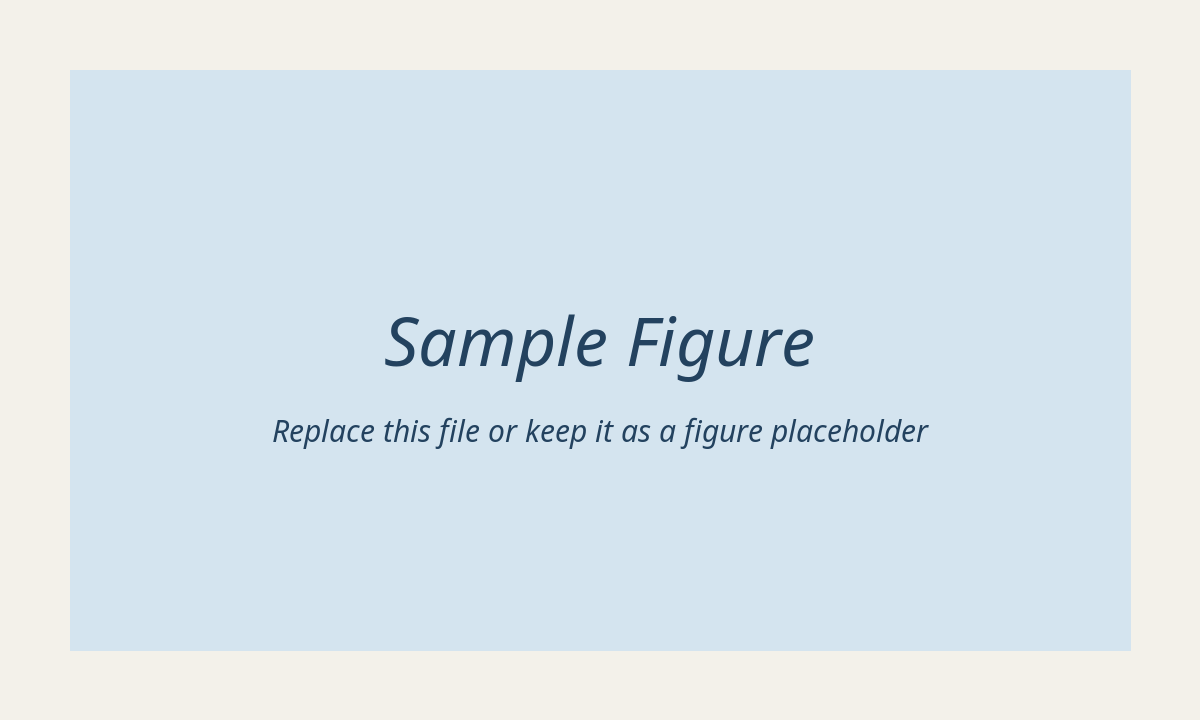
\includegraphics[width=0.72\columnwidth]{pic/example-image.png}
\FigureCaption{画像挿入の例}{fig:method:sample-image}
\end{center}

\begin{BottomColumnBlock}
\begin{center}
\TableCaption{研究スケジュールの例}{tab:method:schedule}
{{\fontsize{9pt}{11pt}\selectfont
\setlength{\tabcolsep}{2.5pt}
\renewcommand{\arraystretch}{1.08}
\begin{tabular}{@{}C{8.5mm}L{61.5mm}@{}}
\hline
\textbf{月} & \multicolumn{1}{c@{}}{\textbf{内容}} \\
\hline
4  & 研究計画書の作成 \\
\hline
5  & \makecell[tl]{関連文献の調査・理解\\先行研究の理解・実装} \\
\hline
6  & 同上 \\
\hline
\end{tabular}}}
\end{center}
\end{BottomColumnBlock}

\subsection{評価方針}\label{sec:method:evaluation}
ここに評価方法や確認項目を書く．
`BottomColumnBlock` の後ろに続く本文は，次の列の先頭から継続する．

\paperreferencesheading
\begin{paperrefs}
\item Reference 1.
\item Reference 2.
\end{paperrefs}

\end{PaperBody}
\end{document}
